\chapter{État de l’existant et cadre théorique}

\section{Introduction}

Ce chapitre présente l’état de l’existant relatif au suivi des opérations terrain du projet Unilever. Il décrit le fonctionnement actuel du processus de reporting, les principales sources de données exploitées, ainsi que les rapports produits à partir des exports issus de la plateforme Smollan.

Il introduit également les notions métier et techniques nécessaires à la compréhension du projet. Ainsi, le chapitre joue un double rôle : présenter l’information existante dans son contexte opérationnel et clarifier les concepts liés au merchandising terrain, aux indicateurs de suivi et à l’exploitation des données.

L’objectif est d’identifier les limites du fonctionnement actuel et de dégager les besoins fonctionnels et techniques auxquels la solution proposée doit répondre. Cette analyse constitue une étape essentielle avant la conception de l’architecture globale du projet.

\section{Cadre théorique du projet}

\subsection{Merchandising terrain et exécution en point de vente}

Le merchandising terrain désigne l’ensemble des actions réalisées en magasin afin d’assurer une bonne présentation des produits et une exécution conforme aux standards définis. Il concerne notamment la disponibilité des produits, leur visibilité en rayon, leur placement, la qualité d’exécution et le respect des consignes commerciales.

Dans le cadre des opérations suivies par Smollan, ces actions sont réalisées par des merchandisers lors des visites en point de vente. Les informations collectées peuvent inclure les réponses aux tâches, les photos justificatives, les relevés liés aux produits, les données de localisation et les éléments nécessaires au reporting. Ces données permettent de vérifier l’état réel de l’exécution terrain et d’alimenter les analyses opérationnelles.

\subsection{Indicateurs de suivi opérationnel}

Le pilotage des opérations de merchandising repose sur plusieurs indicateurs permettant de mesurer l’avancement des visites et la qualité de l’exécution. La couverture permet de suivre les magasins planifiés, visités ou non visités. Les visites exécutées indiquent les interventions effectivement réalisées, tandis que les déviations et les visites rejetées signalent des situations nécessitant une vérification ou une action de suivi.

D’autres indicateurs concernent directement l’exécution commerciale en magasin. L’OSA permet d’évaluer la disponibilité des produits en rayon. Le SOS (\textit{Share of Shelf}) mesure la part de linéaire occupée par une marque ou une catégorie. La qualité d’exécution et le respect du planogramme permettent de vérifier si les produits sont présentés conformément aux standards attendus. Ces indicateurs sont complémentaires, car ils permettent d’analyser à la fois l’avancement terrain et la qualité des actions réalisées.

\subsection{Exploitation des données terrain}

Les données terrain ne peuvent pas être exploitées efficacement lorsqu’elles restent dispersées dans plusieurs fichiers ou rapports séparés. Avant leur utilisation dans des tableaux de bord, une application mobile ou un portail back-office, elles doivent être nettoyées, structurées et centralisées dans un modèle cohérent.

Cette centralisation permet de conserver un historique exploitable, de rapprocher les informations issues de différentes sources et de produire des indicateurs fiables. Elle facilite également la distinction entre les usages internes et les usages orientés client. Les tableaux de bord servent au pilotage et à l’analyse, l’application mobile permet une consultation ciblée des informations par les superviseurs concernés, tandis que le portail back-office reste destiné aux validations et contrôles internes.

Après avoir présenté ces notions générales, il convient d’analyser le fonctionnement actuel du suivi opérationnel afin d’identifier les limites auxquelles la solution proposée doit répondre.
\section{Processus actuel de suivi opérationnel}

Dans le cadre du projet Unilever, le suivi des activités terrain repose initialement sur les données issues de la plateforme opérationnelle utilisée par Smollan. Les merchandisers réalisent leurs visites à travers l’application terrain, dans laquelle ils renseignent les informations liées à l’exécution en magasin : présence au point de vente, tâches réalisées, réponses aux questionnaires, disponibilité des produits, éléments de qualité, photos justificatives et données de localisation.

Le processus actuel s’appuie principalement sur l’extraction quotidienne de fichiers Excel depuis la plateforme Smollan. Ces exports permettent de suivre l’activité de la veille ou d’une période sélectionnée. Les deux fichiers les plus importants dans ce processus sont le fichier \textit{Data Dump} et le fichier \textit{Coverage}. Le premier regroupe les détails d’exécution saisis sur le terrain, tandis que le second apporte une vision plus opérationnelle de la couverture, des visites planifiées, des visites réalisées, des visites adhoc, des rejets, des déviations et des magasins non visités.

Ces fichiers sont exploités pour produire différents reportings. Certains sont orientés vers le suivi interne, notamment les rapports de couverture, de déviation, de visites rejetées et de magasins non visités. D’autres sont destinés au client Unilever, comme le suivi OSA transmis quotidiennement, ainsi que des reportings plus spécifiques ou périodiques liés à la qualité d’exécution, au SOS, au placement en rayon ou à d’autres indicateurs terrain. Ces reportings permettent de suivre l’état d’avancement des opérations, d’analyser la disponibilité des produits, d’identifier les magasins nécessitant un suivi particulier et de faciliter les actions de suivi.

Ce processus permet d’assurer un suivi quotidien des opérations. Toutefois, il reste fortement dépendant des exports Excel et de traitements séparés. Les informations nécessaires à l’analyse sont présentes, mais elles sont dispersées entre plusieurs fichiers et rapports. De plus, le fichier Data Dump ne suffit pas à lui seul pour reconstituer toute la situation opérationnelle, car certaines informations liées aux visites planifiées, non réalisées ou rejetées sont principalement disponibles dans le fichier Coverage. Cette situation rend plus difficile la constitution d’un historique structuré, l’accès rapide aux détails d’exécution d’un magasin et la mise en place d’indicateurs consolidés pour le pilotage opérationnel.


La figure suivante présente une vue simplifiée du processus actuel de reporting, depuis la saisie des informations terrain dans l'application Smart 3 jusqu'à la production des rapports internes et des reportings destinés au client Unilever.

\begin{figure}[H]
    \centering
    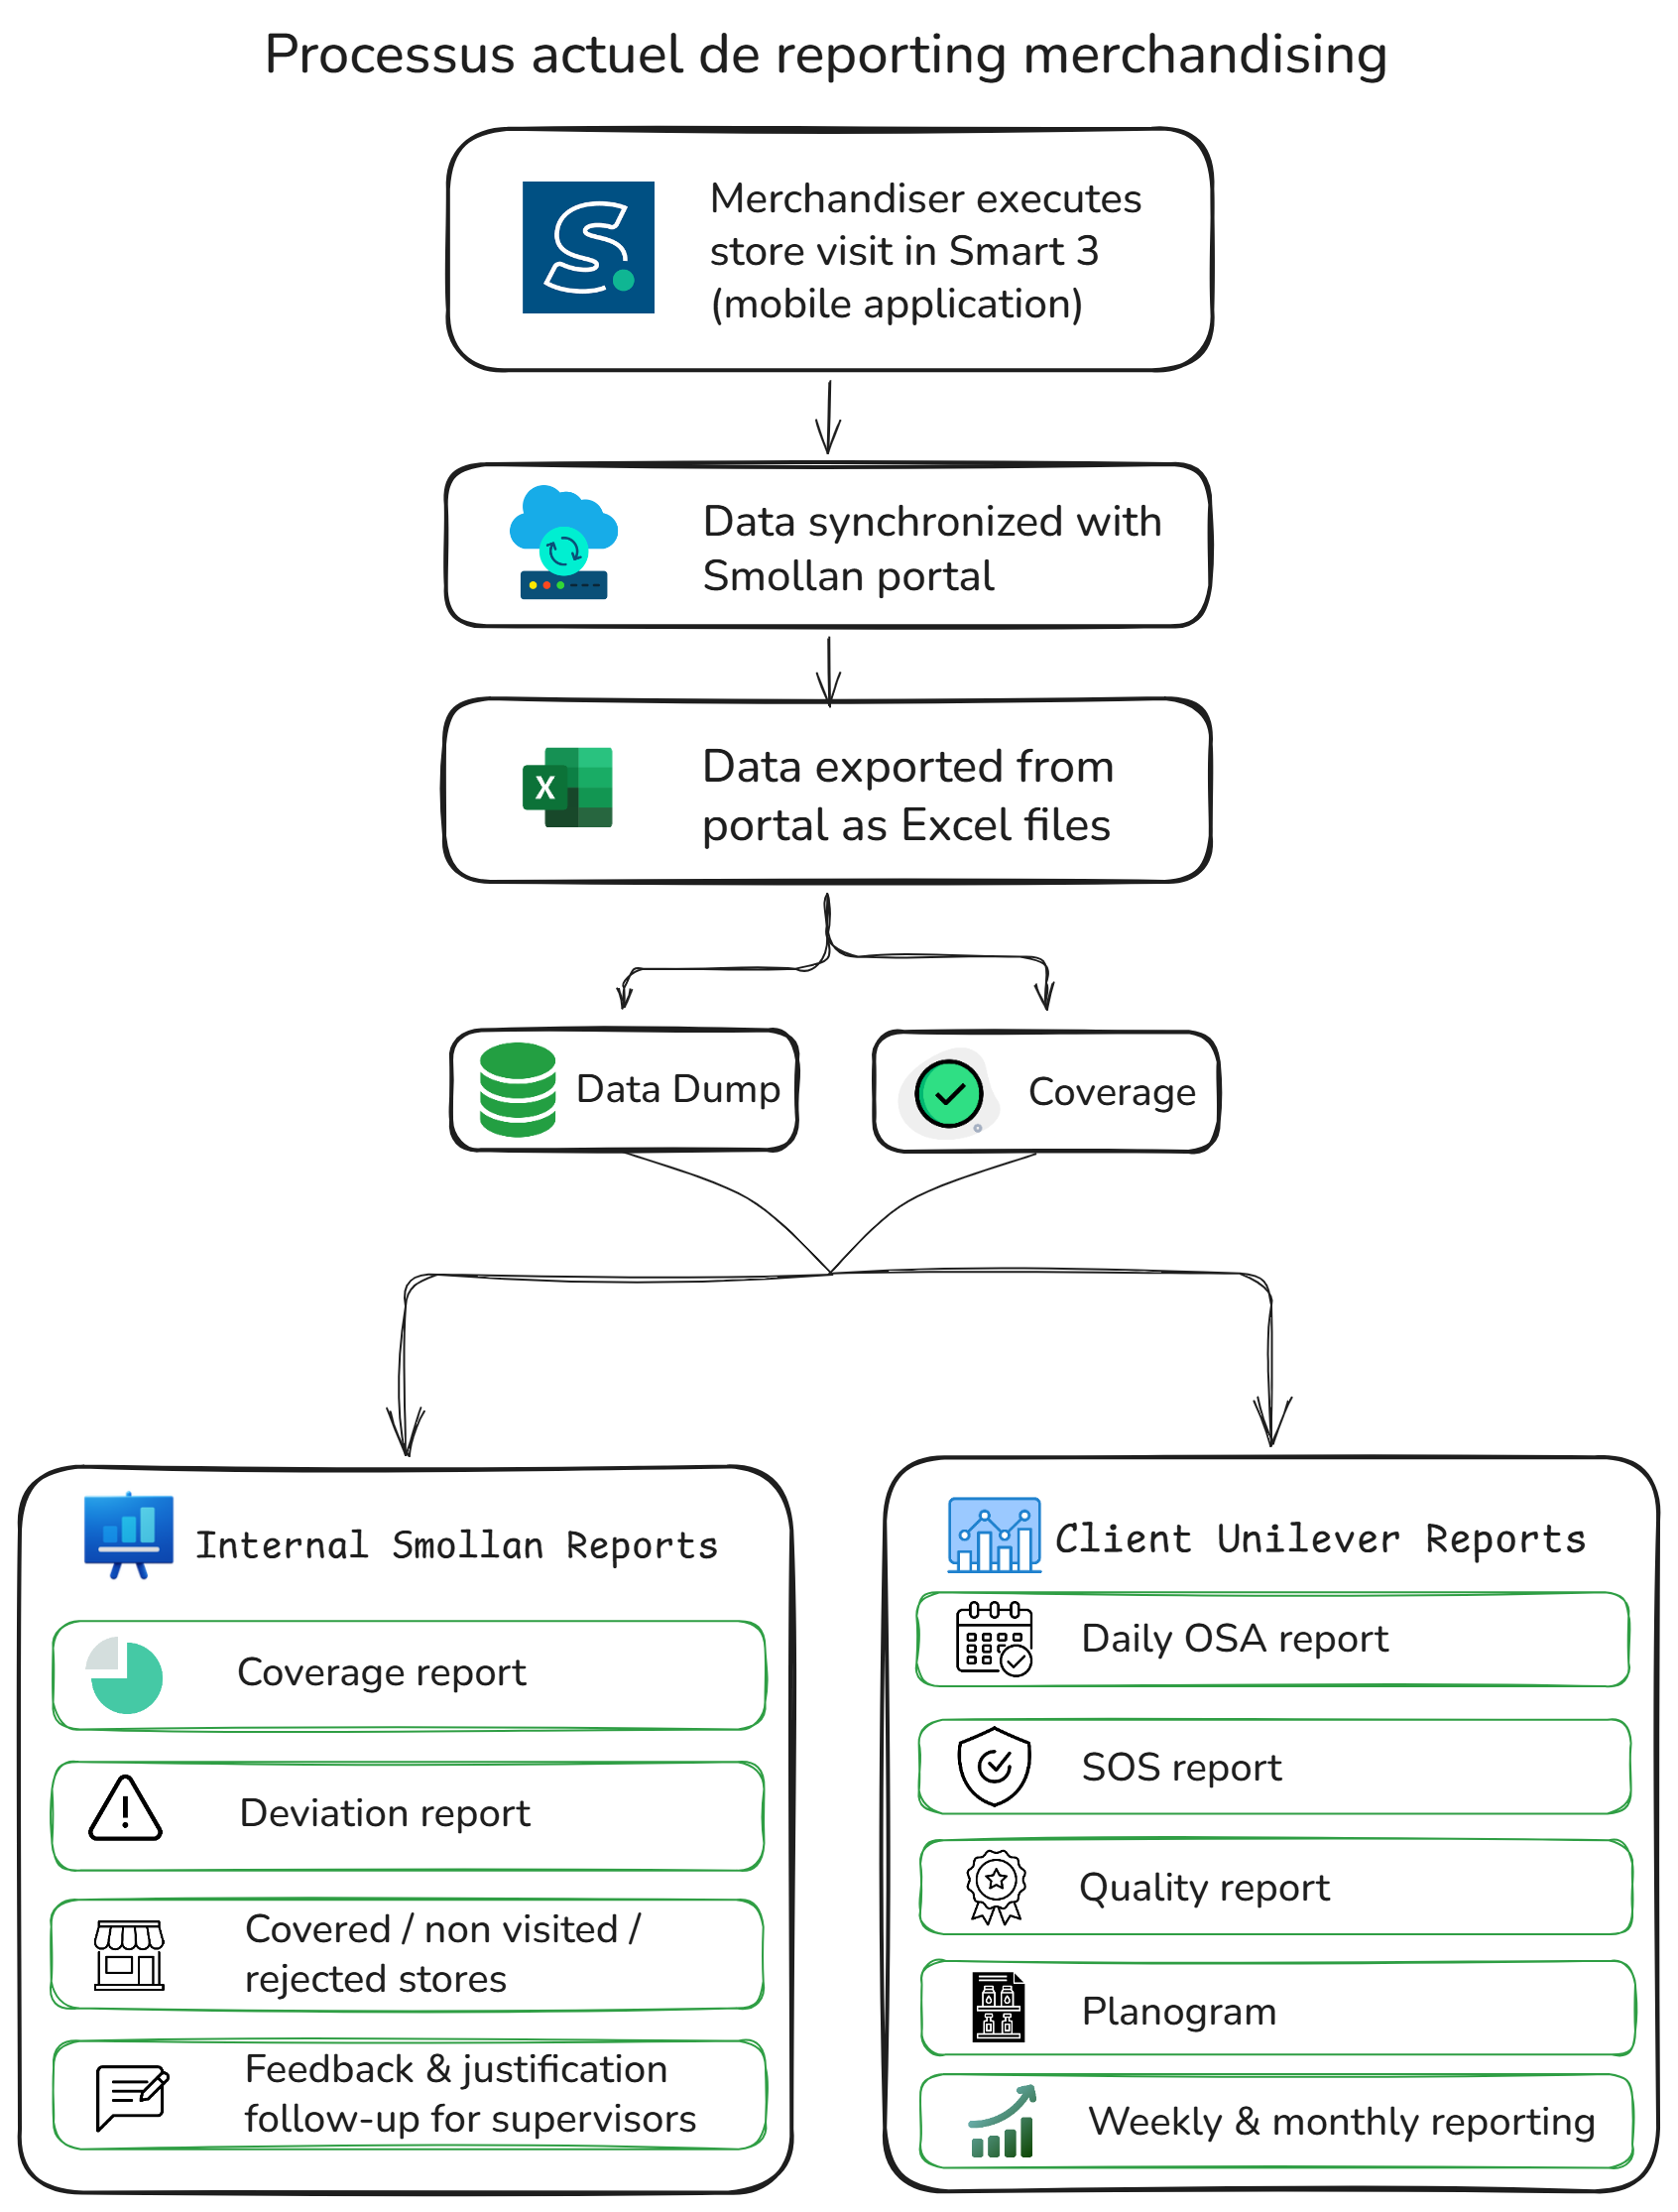
\includegraphics[width=0.85\textwidth]{figures/architecture/Processus_actuel_de_suivi_opérationnel.png}
    \caption{Processus actuel de reporting merchandising basé sur Smart 3 et les exports Excel}
    \label{fig:current-reporting-process}
\end{figure}

Cette figure montre que les exports issus du portail Smollan constituent le point de départ de plusieurs usages. Les rapports internes sont principalement orientés vers le suivi opérationnel, notamment la couverture, les déviations, les rejets et les justifications terrain. Les reportings destinés au client Unilever sont davantage orientés vers la disponibilité produit, la qualité d’exécution, le SOS, le planogramme et les analyses hebdomadaires ou mensuelles.

\section{Sources de données exploitées}

\subsection{Fichier Data Dump}

Le fichier \textit{Data Dump} constitue la source principale des données détaillées issues de l’exécution terrain. Il contient les réponses renseignées par les merchandisers lors de leurs visites en magasin, ainsi que les informations associées aux tâches exécutées.

Ce fichier regroupe notamment les données relatives aux merchandisers, aux magasins, aux produits, aux catégories, aux tâches, aux questions posées et aux réponses saisies. Il contient également des informations liées aux dates d’exécution, aux coordonnées de localisation collectées par l’application terrain et, dans certains cas, aux liens vers les photos justificatives.

Dans le cadre du projet, le \textit{Data Dump} permet d’analyser plusieurs dimensions de l’exécution merchandising, telles que l’OSA, la qualité d’exécution, le placement primaire, le placement secondaire, le SOS, les relevés de prix, les conditions magasin ainsi que les opérations de check-in et check-out. Il représente donc une source riche pour comprendre ce qui a été réellement renseigné sur le terrain.

Toutefois, cette richesse s’accompagne d’une certaine complexité. Les données sont organisées sous forme de lignes de réponses, avec des tâches, des questions et des formats variables selon les cas. Cette structure nécessite un traitement de transformation afin de construire des tables exploitables pour l’analyse, la validation et la restitution dans les tableaux de bord.

\subsection{Fichier Coverage}

Le fichier \textit{Coverage} apporte une vision plus synthétique et opérationnelle de l’activité terrain. Contrairement au \textit{Data Dump}, qui décrit principalement les réponses et les tâches renseignées lors des visites, le fichier \textit{Coverage} permet de suivre l’état des visites prévues et réalisées.

Il contient notamment les informations liées aux visites planifiées, aux visites exécutées, aux visites adhoc, aux visites rejetées, aux déviations, aux magasins non visités, aux merchandisers, aux superviseurs, aux formats de magasins, aux villes, aux régions, ainsi qu’à certaines informations de durée et de localisation.

Ce fichier est essentiel pour le calcul des indicateurs opérationnels, notamment le taux de couverture, le nombre de visites exécutées, les visites non réalisées, les rejets, les déviations et l’activité des merchandisers sur une période donnée. Il permet également d’alimenter les vues de suivi utilisées dans les tableaux de bord et dans l’application mobile.

Ainsi, le fichier \textit{Coverage} joue un rôle central dans la compréhension de l’état d’avancement du terrain, car il permet de relier la planification des visites à leur réalisation effective.

\subsection{Complémentarité Data Dump / Coverage}

Les fichiers \textit{Data Dump} et \textit{Coverage} sont complémentaires. Le \textit{Data Dump} permet d’analyser le contenu détaillé des visites exécutées, tandis que le \textit{Coverage} permet de reconstituer la vision opérationnelle globale des visites planifiées, réalisées, rejetées ou non effectuées.

Cette complémentarité est importante, car l’analyse de l’exécution terrain ne peut pas reposer uniquement sur les réponses détaillées des tâches. Par exemple, un magasin non visité ou une visite rejetée peut ne pas disposer du même niveau de détail dans le \textit{Data Dump}, alors que ces informations sont indispensables pour le suivi opérationnel. Le fichier \textit{Coverage} permet donc de compléter cette lecture en apportant le statut des visites et les informations de couverture.

Dans le cadre de la solution développée, l’exploitation conjointe de ces deux sources permet de construire une base de données plus cohérente. Les données détaillées issues du \textit{Data Dump} alimentent les tables de tâches et les réponses normalisées, tandis que les données du \textit{Coverage} alimentent les indicateurs de suivi opérationnel. Cette approche permet d’obtenir une vision à la fois détaillée et globale des activités terrain.


Le tableau suivant synthétise le rôle de chaque source dans la solution proposée.

\begin{table}[H]
\centering
\caption{Comparaison entre les fichiers Data Dump et Coverage}
\label{tab:data-dump-coverage}
\renewcommand{\arraystretch}{1.25}
\small
\begin{tabular}{
|>{\raggedright\arraybackslash}p{2.8cm}
|>{\raggedright\arraybackslash}p{4cm}
|>{\raggedright\arraybackslash}p{4cm}
|>{\raggedright\arraybackslash}p{4cm}|
}
\hline
\textbf{Fichier} & \textbf{Type d'information} & \textbf{Utilité dans le projet} & \textbf{Limite principale} \\
\hline
\textit{Data Dump}
& Données détaillées d'exécution terrain : tâches, questions, réponses, produits, photos et informations de localisation.
& Analyse du contenu des visites réalisées : réponses OSA, qualité d'exécution, placement en rayon, SOS et autres tâches terrain.
& Ne permet pas à lui seul de reconstituer toute la situation opérationnelle, notamment les visites non réalisées ou certains statuts de couverture. \\
\hline
\textit{Coverage}
& Données de suivi opérationnel : visites planifiées, visites réalisées, visites adhoc, rejets, déviations, magasins non visités et informations de supervision.
& Calcul des KPI de couverture, suivi de l'avancement terrain et alimentation des vues de pilotage opérationnel.
& Ne fournit pas toujours le détail complet des réponses terrain et des tâches exécutées, principalement disponibles dans le \textit{Data Dump}. \\
\hline
\end{tabular}
\end{table}

Cette comparaison montre que les deux fichiers répondent à des besoins différents. Le \textit{Data Dump} apporte le détail de l'exécution terrain, tandis que le \textit{Coverage} permet de suivre l'état global des visites. Leur combinaison constitue donc une base nécessaire pour construire une lecture fiable des opérations.


\section{Rapports existants}

Les fichiers exportés depuis la plateforme Smollan servent de base à plusieurs reportings utilisés dans le suivi des opérations terrain. Ces reportings peuvent être regroupés en deux grandes catégories : les rapports destinés au suivi interne des opérations et les rapports destinés au client Unilever.

\subsection{Rapports internes Smollan}

Les rapports internes sont principalement orientés vers le suivi opérationnel quotidien. Ils permettent de suivre l’état de couverture, les visites réalisées, les visites non effectuées, les déviations, les rejets et certains éléments liés à l’assiduité ou au temps de production. Ces rapports facilitent la lecture de l’activité terrain et permettent d’identifier les situations nécessitant un suivi opérationnel.

Parmi les rapports internes les plus utilisés, on retrouve notamment les rapports de couverture et les rapports de déviation. Le rapport de couverture permet d’obtenir une vision de l’avancement des visites, tandis que le rapport de déviation met en évidence les magasins nécessitant une confirmation, une justification ou une revisite selon le contexte terrain.

Ces reportings jouent donc un rôle important dans la coordination quotidienne des opérations. Toutefois, ils restent généralement produits sous forme de fichiers séparés, ce qui limite l’analyse historique et la centralisation des informations dans une seule base exploitable.

\subsection{Rapports destinés au client Unilever}

En parallèle des rapports internes, certaines restitutions sont destinées au client Unilever. Elles concernent principalement la qualité d’exécution en magasin, la disponibilité des produits et certains indicateurs liés à la visibilité ou à la présence des produits en rayon.

Le suivi OSA constitue un exemple important de reporting client, car il permet d’analyser la disponibilité des produits dans les magasins visités. D’autres reportings, comme les rapports liés à la qualité d’exécution, au SOS, au placement en rayon ou à d’autres indicateurs terrain, peuvent être produits de manière périodique ou selon les besoins du suivi opérationnel.

Ces rapports permettent au client de disposer d’une lecture sur l’exécution terrain et sur les points nécessitant une attention particulière. Cependant, comme pour les rapports internes, leur exploitation reste dépendante des fichiers sources et des traitements réalisés en amont.

Le tableau suivant résume les principaux types de reportings produits à partir des fichiers opérationnels.

\begin{table}[H]
\centering
\caption{Synthèse des reportings existants}
\label{tab:reportings-existants}
\renewcommand{\arraystretch}{1.25}
\small
\begin{tabular}{
|>{\raggedright\arraybackslash}p{3.2cm}
|>{\raggedright\arraybackslash}p{3.2cm}
|>{\raggedright\arraybackslash}p{3cm}
|>{\raggedright\arraybackslash}p{5cm}|
}
\hline
\textbf{Type de rapport} & \textbf{Destinataire} & \textbf{Fréquence} & \textbf{Objectif principal} \\
\hline
Rapport de couverture
& Suivi interne
& Quotidienne
& Suivre l’avancement des visites, les magasins couverts, les magasins non visités et l’état global du terrain. \\
\hline
Rapport de déviation
& Suivi interne
& Quotidienne ou selon le besoin
& Identifier les magasins nécessitant une confirmation, une justification ou une action de suivi. \\
\hline
Suivi OSA
& Client Unilever
& Quotidienne
& Suivre la disponibilité des produits et identifier les références non disponibles en magasin. \\
\hline
Rapports qualité, SOS et placement
& Client Unilever
& Périodique ou selon le besoin
& Analyser la qualité d’exécution, la présence produit, le placement en rayon et les points nécessitant une attention particulière. \\
\hline
\end{tabular}
\end{table}

Ce tableau montre que les reportings existants répondent à des besoins complémentaires. Les rapports internes soutiennent le pilotage quotidien des opérations, tandis que les reportings destinés au client permettent de suivre la disponibilité, la qualité d’exécution et la visibilité des produits en magasin.

\section{Limites du processus actuel}

Le processus actuel permet d'assurer un suivi quotidien des opérations terrain, mais il présente plusieurs limites lorsque les volumes de données augmentent et lorsque les besoins d'analyse deviennent plus avancés. La première limite concerne la dépendance aux fichiers Excel exportés depuis la plateforme. Ces fichiers restent indispensables au suivi opérationnel, mais leur exploitation sous forme de rapports séparés rend plus difficile la centralisation de l'information et la construction d'une vision historique consolidée.

La deuxième limite concerne la dispersion des données entre plusieurs sources. Le fichier \textit{Data Dump} contient les détails d'exécution, tandis que le fichier \textit{Coverage} apporte les informations de couverture et de statut des visites. Cette complémentarité est nécessaire, mais elle impose un travail de rapprochement afin de produire des indicateurs fiables. Sans modèle de données centralisé, l'analyse peut devenir répétitive et dépendante de traitements manuels ou semi-automatisés.

Une autre limite concerne l'accès aux détails d'exécution par magasin. Les rapports existants permettent de suivre l'état global des opérations, mais l'accès rapide à l'historique d'un magasin, aux tâches exécutées, aux réponses terrain ou aux éléments justificatifs reste moins direct. Cette situation limite la capacité à consulter facilement une vision détaillée et structurée de l'exécution terrain.

Enfin, les besoins de suivi ne sont pas identiques selon les utilisateurs. Les équipes internes ont besoin d'indicateurs de pilotage, de contrôle et de validation opérationnelle, tandis que les superviseurs côté client doivent disposer d'une consultation plus ciblée sur les magasins qui leur sont affectés. Cette différence d'usage montre la nécessité de distinguer les couches de restitution : tableaux de bord BI pour le pilotage, application mobile client pour la consultation des magasins affectés, et portail back-office pour le suivi interne des validations.

\section{Besoins fonctionnels}

À partir des limites identifiées dans le processus actuel, plusieurs besoins fonctionnels ont été définis afin de structurer la solution proposée. Ces besoins concernent à la fois la centralisation des données, le suivi des indicateurs opérationnels, la consultation des informations terrain et la validation interne des situations nécessitant une analyse complémentaire.

Le premier besoin consiste à mettre en place une base de données centralisée capable de regrouper les informations issues des fichiers \textit{Data Dump} et \textit{Coverage}. Cette base doit permettre de conserver l'historique des données, de structurer les informations relatives aux visites, aux magasins, aux merchandisers, aux produits et aux tâches exécutées, et de faciliter leur exploitation dans les différentes couches de la solution.

Le deuxième besoin concerne la mise à disposition de tableaux de bord décisionnels permettant de suivre l’avancement des opérations terrain et d’analyser les principaux indicateurs avant la restitution finale. Ces dashboards doivent aider au pilotage interne et au management, tout en facilitant la lecture des données liées à la couverture, à l’activité des merchandisers et à certains reportings client comme l’OSA, la qualité d’exécution, le SOS ou le placement en rayon.

Le troisième besoin concerne le développement d'une application mobile orientée client. Cette application doit permettre aux superviseurs côté Unilever de se connecter et de consulter uniquement les magasins qui leur sont affectés. L'objectif est de leur offrir une visibilité simple et ciblée sur l'exécution terrain, les informations des magasins, les dernières visites et les détails liés aux tâches exécutées.

Le quatrième besoin porte sur la mise en place d'un portail back-office interne destiné au suivi des validations opérationnelles. Ce portail doit permettre d'exploiter les résultats des règles de validation, notamment les cas liés à l'OSA, aux contrôles GPS ou à d'autres situations nécessitant une vérification. Il doit constituer un espace interne de consultation, d'analyse et, à terme, de suivi des actions correctives.

Ainsi, les besoins fonctionnels du projet ne se limitent pas à la production de tableaux de bord. Ils couvrent l'ensemble de la chaîne d'exploitation de la donnée, depuis l'ingestion des fichiers jusqu'à la restitution des informations sous forme de dashboards, d'application mobile client et de portail de validation interne.


\section{Besoins techniques}

La mise en œuvre de la solution nécessite une architecture technique capable de traiter des fichiers Excel volumineux, de structurer les données et de les rendre exploitables par plusieurs outils. Le premier besoin technique concerne la mise en place d’un pipeline ETL développé en Python, permettant d’extraire, nettoyer, transformer et charger les données issues des fichiers \textit{Data Dump} et \textit{Coverage}.

Le deuxième besoin concerne la centralisation des données dans une base MySQL. Cette base doit permettre de stocker les informations opérationnelles, les réponses terrain, les tables liées aux différentes tâches, ainsi que les indicateurs nécessaires aux tableaux de bord, à l’application mobile et au portail de validation.

Le troisième besoin porte sur la restitution et l’intégration des données. Les tableaux de bord sont réalisés avec Power BI afin de faciliter l’analyse et le pilotage des indicateurs. L’application mobile client et le portail back-office nécessitent une couche backend exposant des APIs, développée avec Spring Boot, afin de communiquer avec la base de données et de fournir les informations aux interfaces React.

Enfin, la solution doit rester évolutive afin de permettre l’ajout progressif de nouvelles règles de validation, de nouvelles vues analytiques, de nouveaux fichiers sources comme les Masters, ainsi que des mécanismes d’authentification et de gestion des rôles plus avancés.

\section{Conclusion}

Ce chapitre a permis d’introduire les notions nécessaires à la compréhension du projet, notamment le merchandising terrain, les indicateurs de suivi opérationnel et l’exploitation structurée des données collectées en magasin. Ces éléments théoriques ont posé le cadre métier et technique dans lequel s’inscrit la solution proposée.

L’état de l’existant a ensuite permis d’analyser le fonctionnement actuel du suivi des opérations terrain dans le cadre du projet Unilever. L’étude du processus actuel a montré que les fichiers \textit{Data Dump} et \textit{Coverage} constituent deux sources complémentaires : le premier apporte le détail de l’exécution terrain, tandis que le second permet de suivre la couverture et le statut opérationnel des visites.

L’analyse des rapports existants a également mis en évidence la diversité des usages des données, entre le suivi interne des opérations et les reportings destinés au client Unilever. Malgré l’utilité de ce fonctionnement, plusieurs limites ont été identifiées, notamment la dépendance aux fichiers Excel, la dispersion des informations, la difficulté de constituer un historique centralisé et la nécessité d’adapter les restitutions selon les utilisateurs.

Ces constats ont permis de définir les principaux besoins fonctionnels et techniques du projet. Ils justifient la mise en place d’une solution data-driven reposant sur une base de données centralisée, des tableaux de bord décisionnels, une application mobile client et un portail back-office de validation interne. Le chapitre suivant présentera la conception globale de cette solution ainsi que son architecture fonctionnelle et technique.
